\section{Context}
This thesis is the product of the participation of a team of students to a robotic contest named RoboCup.

This contest is divided into several leagues :
\begin{itemize}
\item RoboCup Industrial : a category for more industrially focused contests.
\item RoboCup@Home : a league for domestic robots that support elder people and stuff.
\item RoboCupJunior : more of an initiative that aims to foster robotics interest in children, it helps organize various events for younger minds.
\item RoboCup Soccer : historically the first category, centered about humanoid robots playing football in small teams. This is the league we will compete in.
\end{itemize}
The Robocup Soccer league is further divided into several categories :\begin{itemize}
\item Adultsize, for the taller robots
\item Teensize, for middle sized robots
\item Kidsize, for the smaller robots. This is the competition we will join.
\end{itemize}

Us participating to that means that for the first time at the Montefiore Institute, a humanoid robot will be built.

\begin{figure}[htp]
\center
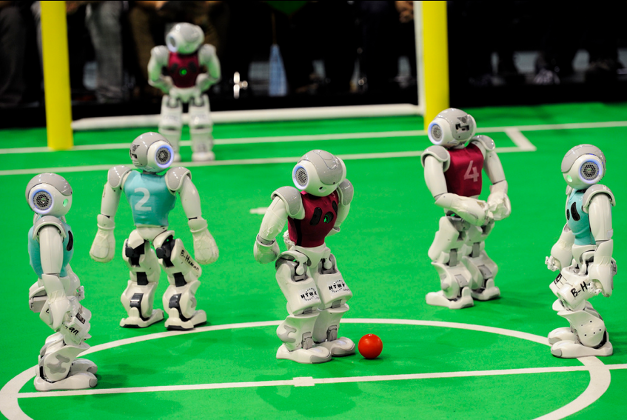
\includegraphics[width=0.5\textwidth]{figures/robocup}
\caption[Two teams of Nao robots playing against each other]{Two teams of Nao robots playing against each other in the 2014 edition of RoboCup \textit{[Photo courtesy of RoboCup]}}
\label{fig:intro_robocup}
\end{figure}

We thus need a reliable simulation tool to :
\begin{enumerate}
\item Test different robot designs and choose the best one, faster than it would be done by building the designs in real life.
\item At a later stage, be able to test control algorithms faster because the real robot is not needed.
\end{enumerate}

\section{Goals of the project}
The goal of this thesis is to provide the team with a simulation tool and a model able of :
\begin{itemize}
\item realistically simulating the dynamics of the robot including springs and dampers
\item receiving orders at approximately 300Hz, and we don't really care if the simulation is not in real time.
\item the simulated robot receives exactly the same orders as the real robot would.
\item visualization
\end{itemize}

\section{Structure of the report}
The report will begin with an overview of the available simulation tools and a choice for this project.

The next chapter will detail the chosen tools. The third chapter will be about tuning and verifying the accurateness of the simulation.

The fourth chapter will show some simulation examples and explain how they influence the design of the robot.

The last chapter will be the conclusion where the work will be summed up and future work prospects laid out.